\documentclass{article}
\usepackage[ruled,vlined,linesnumbered]{algorithm2e}
\usepackage{algpseudocode}
\usepackage{amsmath}
\usepackage{amsthm}
\usepackage{graphicx}
\usepackage{subfigure}
\usepackage{float}
\usepackage{amsmath }
\usepackage{amsfonts }
\usepackage{pdfpages}
\usepackage{epsfig}
\usepackage{graphicx}
\usepackage{arydshln}
\usepackage{verbatim}
\usepackage{subfigure}
\usepackage{enumerate}
\usepackage{rotating}
\usepackage{threeparttable}
\usepackage{caption}
\usepackage{epsfig}
\usepackage{cite}
\usepackage{times}
\usepackage{geometry}
\usepackage{tikz}
\geometry{a4paper}
\renewcommand{\baselinestretch}{1.5}
\usepackage[colorlinks,linkcolor=blue]{hyperref}
\begin{document}
\title{AI3602 Data Mining Homework 2.2}
\author{Kailing Wang 521030910356}
\date{April 26.2024}
\maketitle

\section*{Question 1}
Let $\{i\}\cup C \rightarrow C'$, and similarly for $k_i^{(in)'}$ and other notations.

We have already 
\[
	Q_d(C) = \frac{1}{m} \sum_i \sum_j \left[A_{ij} - \frac{k_i^{(in)}\cdot k_j^{(out)}}{m}\right]\delta (c_i, c_j) = \frac{\Sigma_{(in)}}{m} - \frac{\Sigma_{tot}^{{in}}\cdot\Sigma_{tot}^{(out)}}{m^2}
\]

and $Q_d{\{i\}} = \frac{1}{m} A_{ii} - \frac{1}{m}\frac{k_i^{(in)}\cdot k_i^{(out)}}{m} = -\frac{k_i^{(in)}\cdot k_i^{(out)}}{m^2}$ is naive.

We'd focus on $Q_d(C')$, 
\[
	Q_d(C') = \frac{1}{m} \sum_i \sum_j \left[A_{ij} - \frac{k_i^{(in)'}\cdot k_j^{(out)'}}{m}\right]\delta (c_i, c_j) = \frac{m\Sigma_{(in)}^{'} - \Sigma_{tot}^{(in)'}\cdot\Sigma_{tot}^{(out)'}}{m^2}.
\]

In the above quation, accoridng to $\{i\}\cup C \rightarrow C'$, 
\begin{align*}
	\Sigma_{(in)}^{'}     & = \Sigma_{(in)} + k_{i, in}           \\
	\Sigma_{tot}^{(in)'}  & = \Sigma_{tot}^{(in)} + k_i^{(in)}     \\
	\Sigma_{tot}^{(out)'} & = \Sigma_{tot}^{(out)} + k_i^{(out)}.
\end{align*}

Thus,
\begin{align*}
	\Delta Q_d(i \rightarrow C) & = \frac{m\Sigma_{(in)}^{'} - \Sigma_{tot}^{(in)'}\cdot\Sigma_{tot}^{(out)'}}{m^2} - \frac{\Sigma_{(in)}}{m} - \frac{\Sigma_{tot}^{{in}}\cdot\Sigma_{tot}^{(out)}}{m^2} + \frac{k_i^{(in)}\cdot k_i^{(out)}}{m^2} \\
	                            & = \frac{\Sigma_{(in)}^{'}-\Sigma_{(in)}}{m} - \frac{\Sigma_{tot}^{(in)'}\cdot\Sigma_{tot}^{(out)'} - \Sigma_{tot}^{{in}}\cdot\Sigma_{tot}^{(out)}}{m^2} + \frac{k_i^{(in)}\cdot k_i^{(out)}}{m^2}                \\
	                            & = \frac{k_{i, in}}{m} - \frac{(\Sigma_{tot}^{(in)} + k_i^{(in)})\cdot(\Sigma_{tot}^{(out)} + k_i^{(out)}) - \Sigma_{tot}^{{in}}\cdot\Sigma_{tot}^{(out)}}{m^2} + \frac{k_i^{(in)}\cdot k_i^{(out)}}{m^2}        \\
	                            & = \frac{k_{i, in}}{m} - \frac{k_i^{(in)}\cdot\Sigma_{tot}^{(out)} + k_i^{(out)}\cdot\Sigma_{tot}^{(in)} + k_i^{(in)}\cdot k_i^{(out)}}{m^2} + \frac{k_i^{(in)}\cdot k_i^{(out)}}{m^2}                           \\	
	                            & = \frac{k_{i, in}}{m} - \frac{k_i^{(in)}\cdot\Sigma_{tot}^{(out)} + k_i^{(out)}\cdot\Sigma_{tot}^{(in)}}{m^2}.		
\end{align*}

\section*{Original Questions}
\begin{figure}[h!]
	\centering
	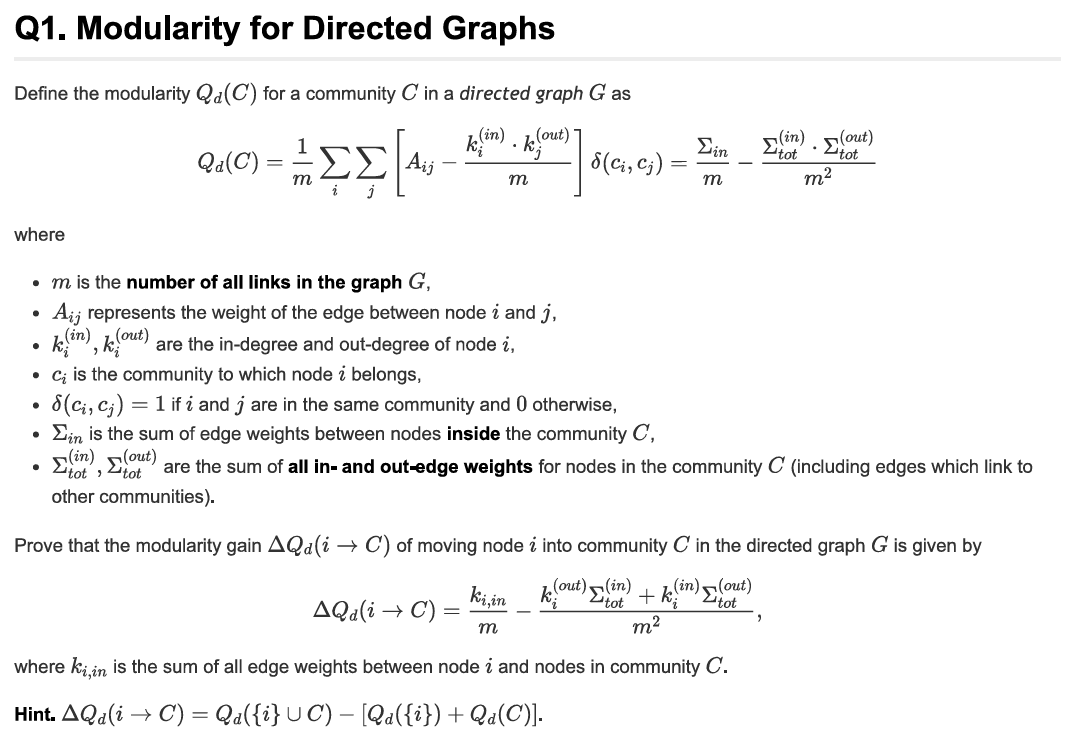
\includegraphics[width=1\textwidth]{preview}
	\caption{Question 1}
	\label{fig:1}
\end{figure}
\section*{Reference}
None.
\end{document}
